\section{Bootstrapping for Uncertainty Estimation and Reduction}
\label{sec:bootstrapping}
\begin{figure*}[t]
	\centering
	\begin{subfigure}[b]{0.23\linewidth}
		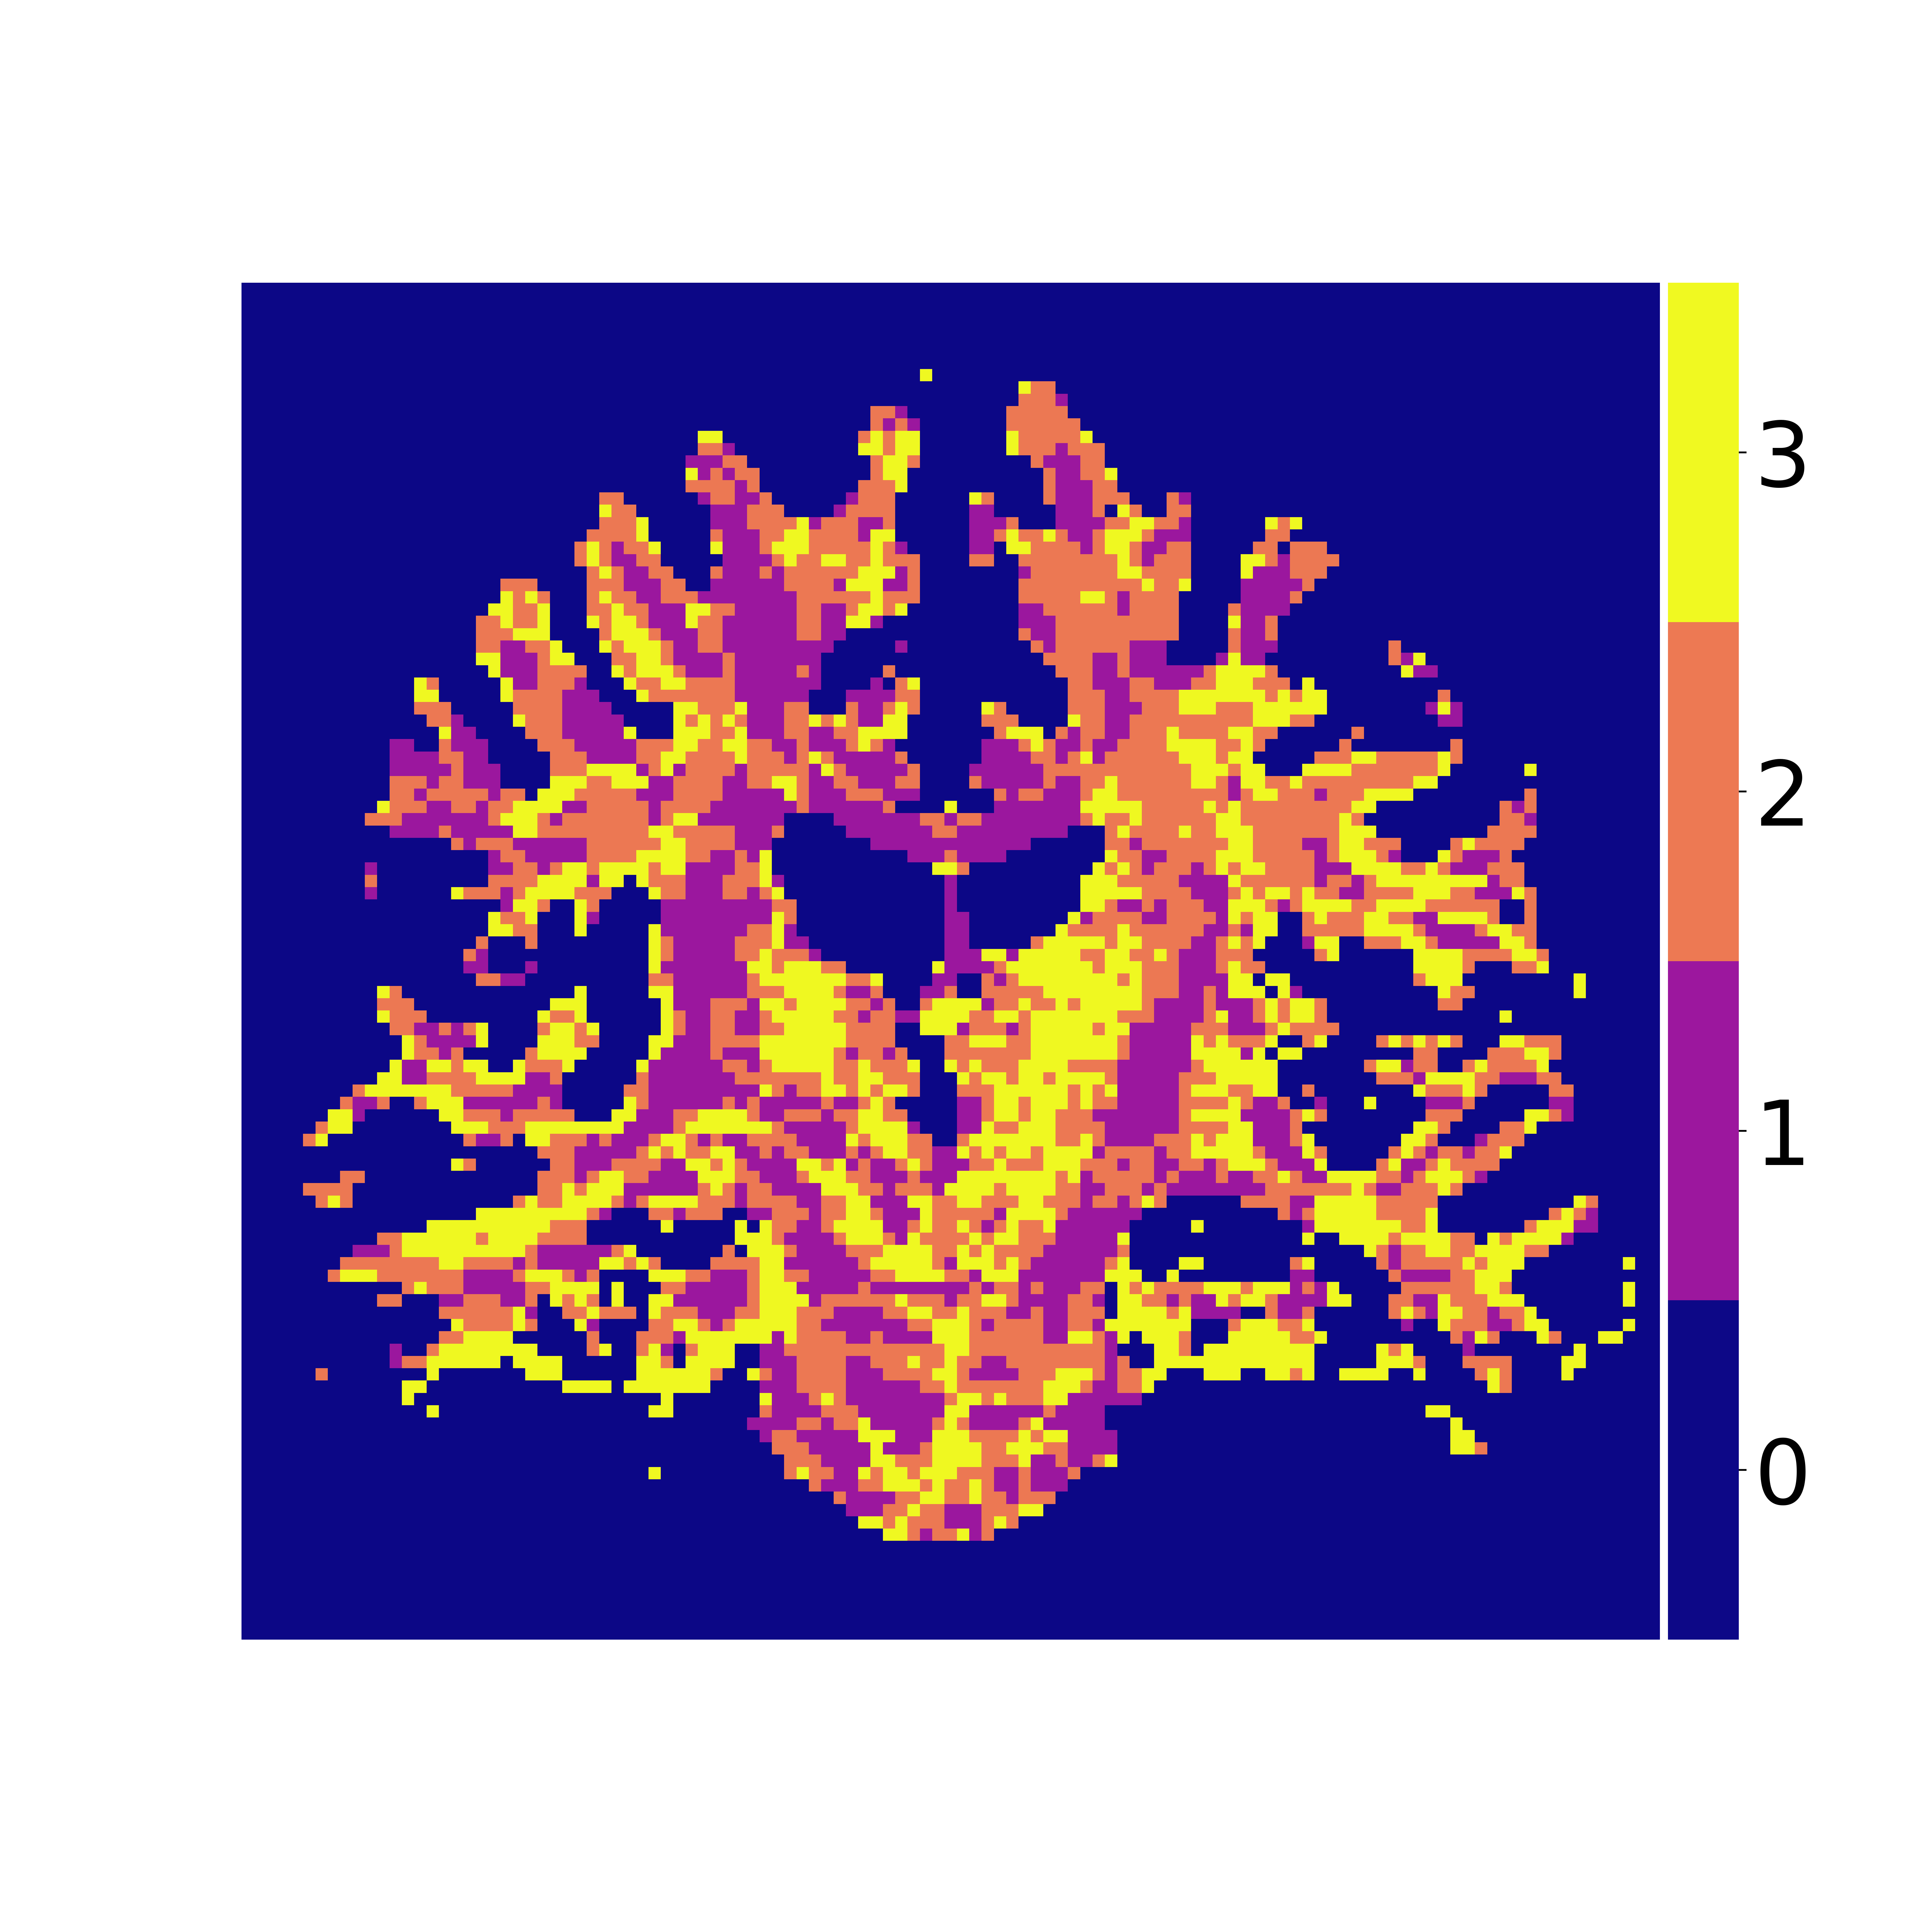
\includegraphics[width=\linewidth]{selected}
		\caption{The most likely number of fibers according to our model
		selection.}
		\label{fig:selected-uncertainty:rank-original}
              \end{subfigure}
              \hspace{0.01\linewidth}
	\begin{subfigure}[b]{0.23\linewidth}
		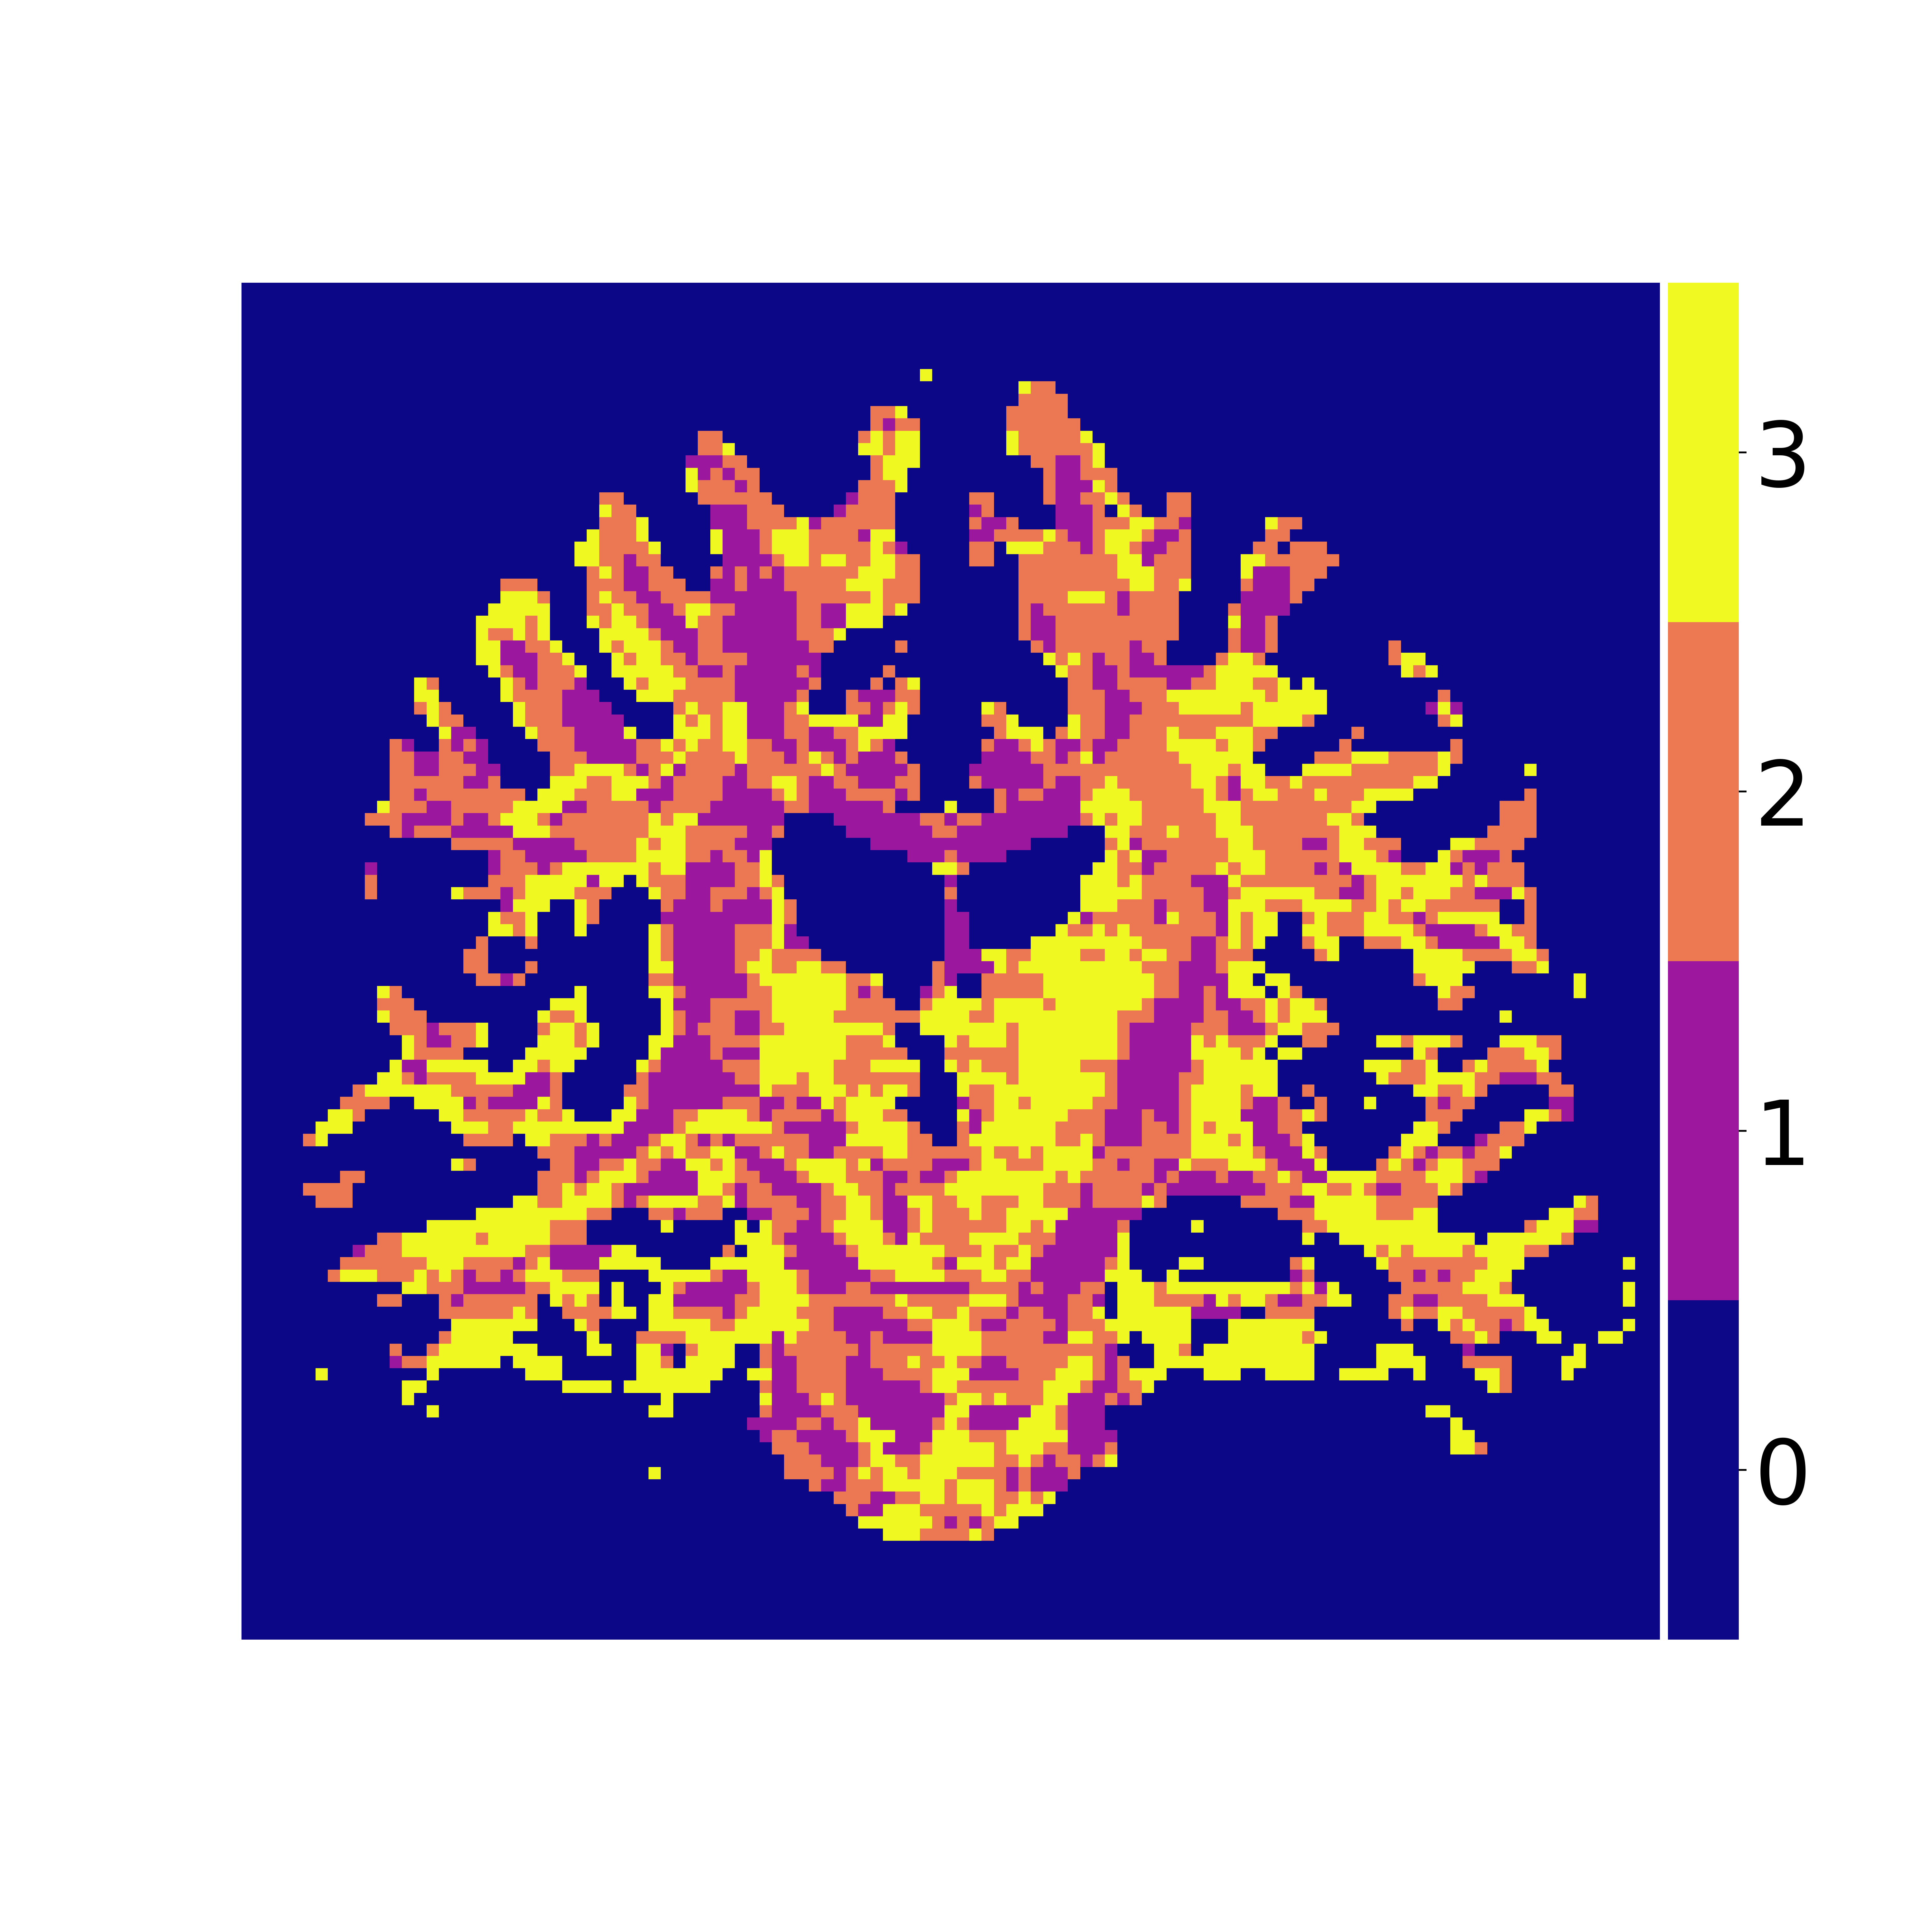
\includegraphics[width=\linewidth]{selected-bootstrap}
		\caption{The most likely number of fibers over all
		bootstraps.}
		\label{fig:selected-uncertainty:rank}
              \end{subfigure}
              \hspace{0.01\linewidth}
	\begin{subfigure}[b]{0.23\linewidth}
		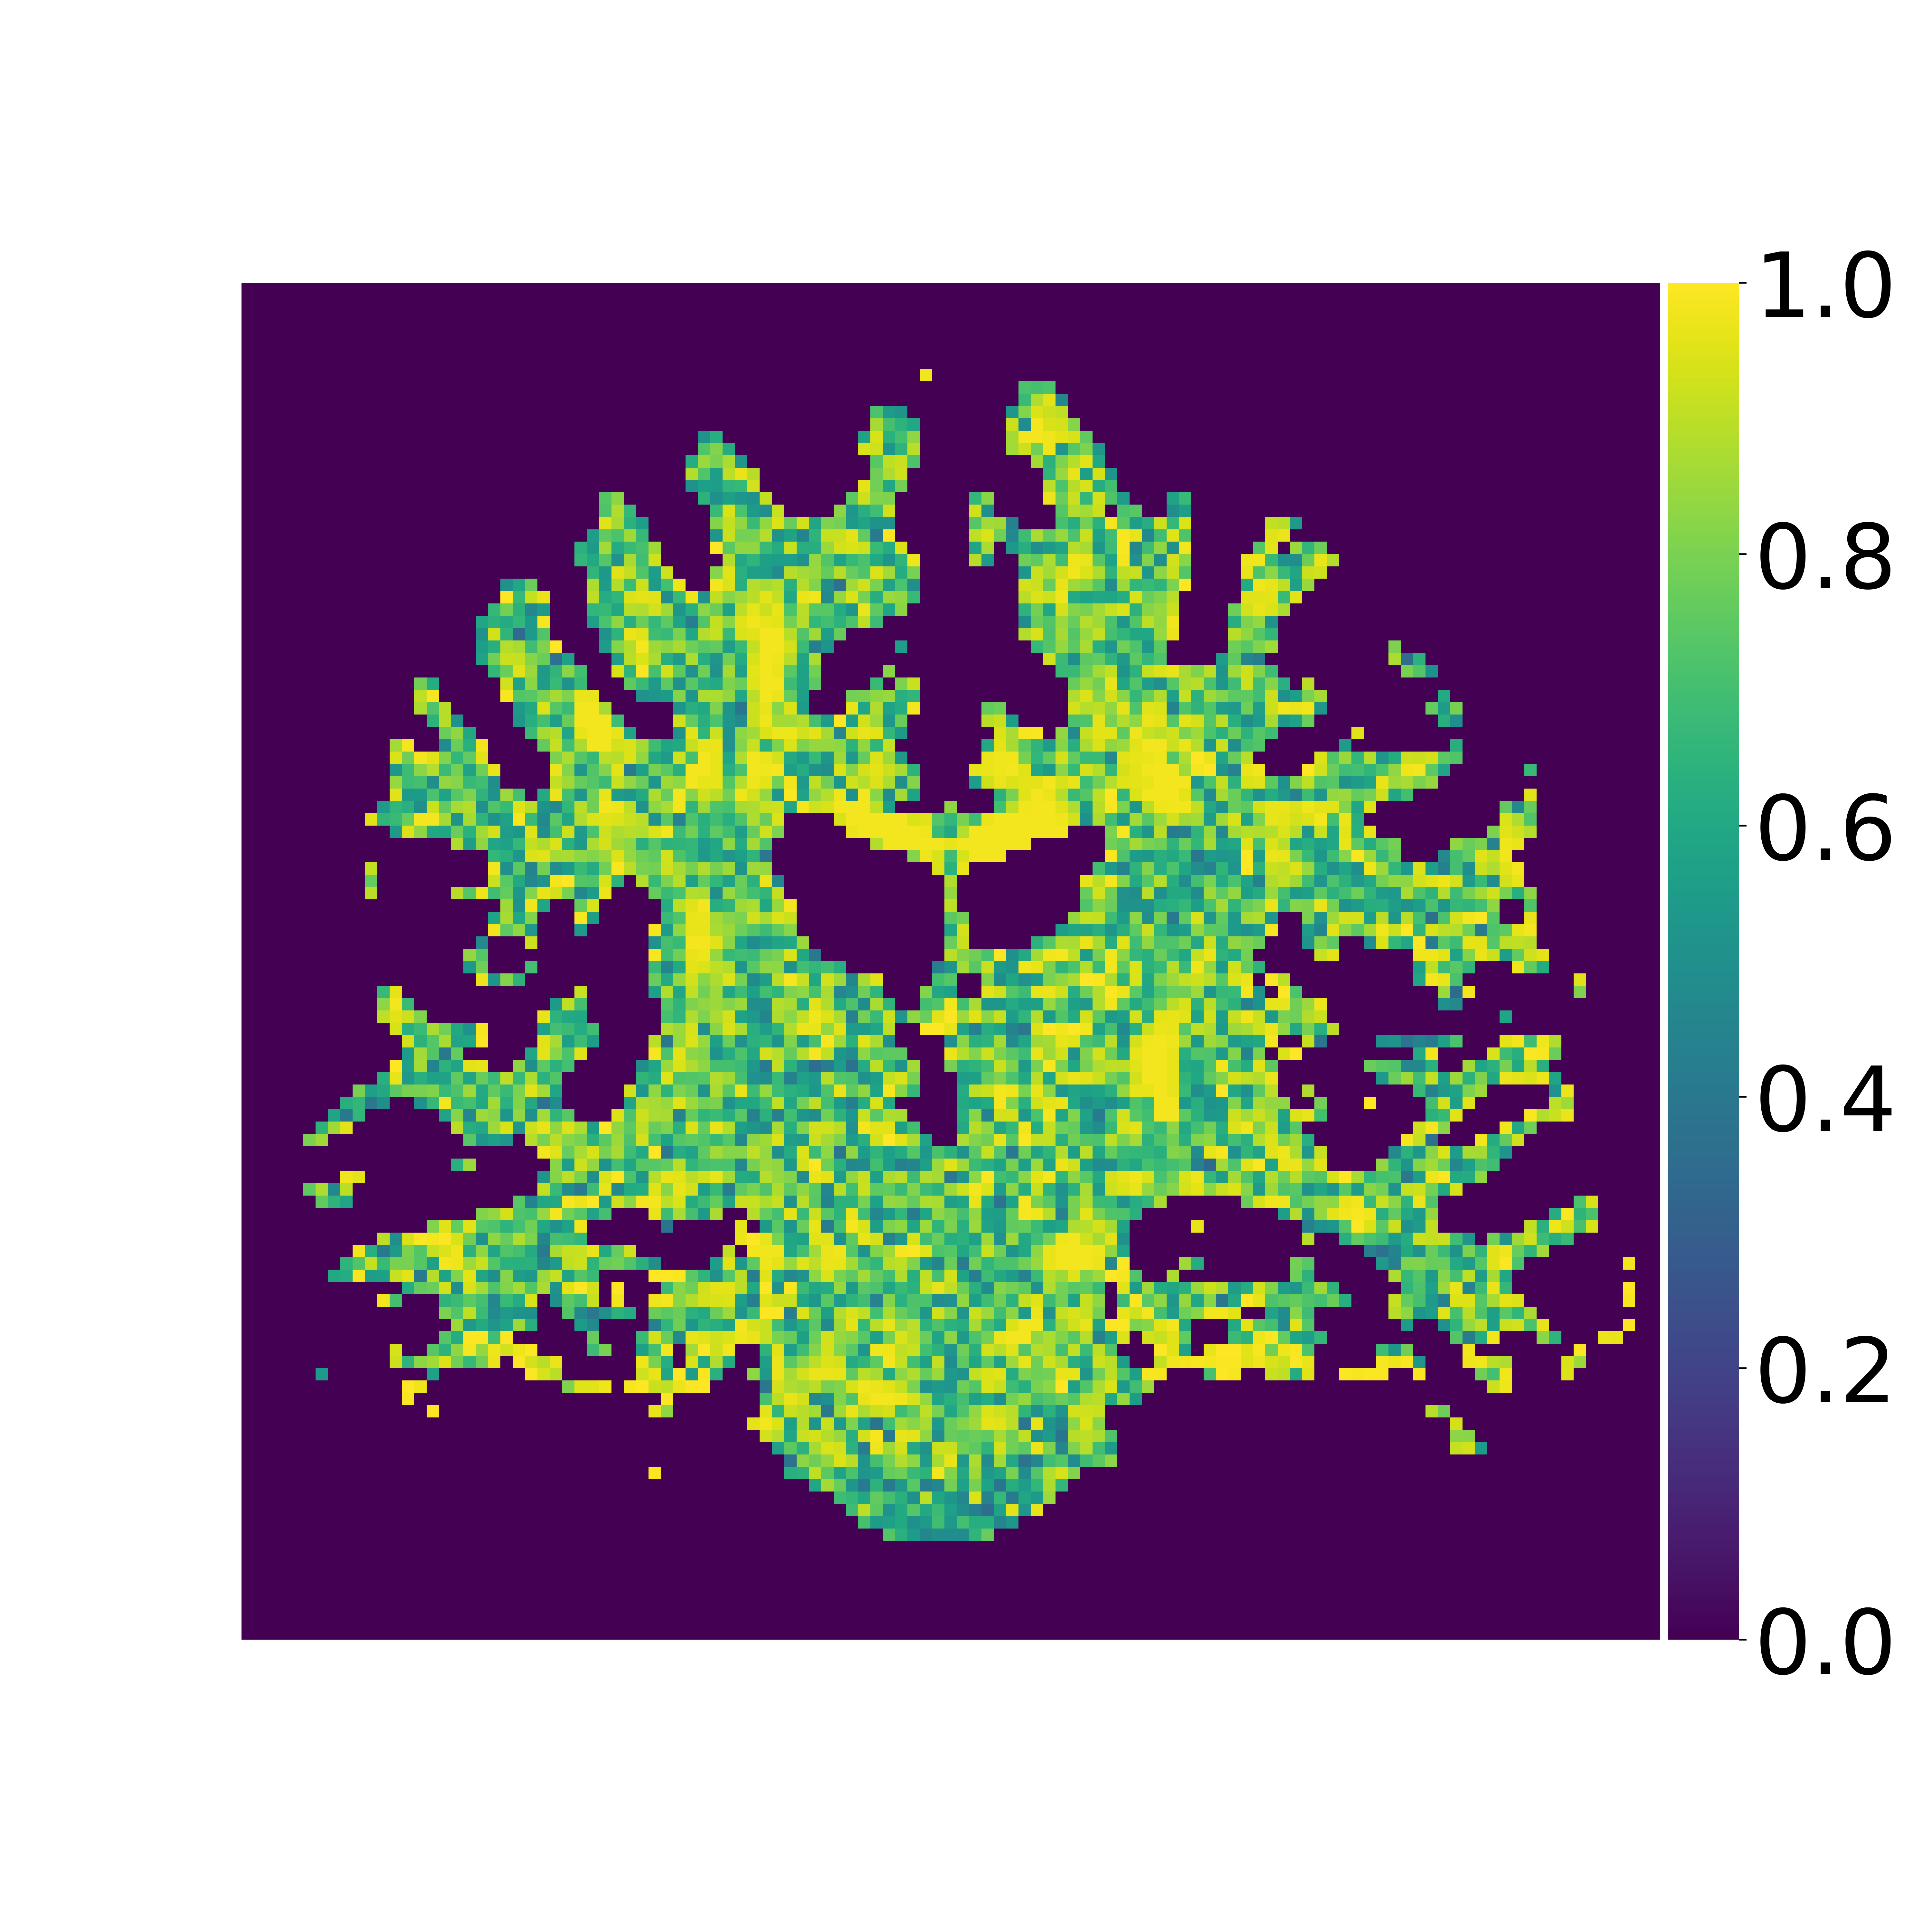
\includegraphics[width=\linewidth]{uncertainty}
		\caption{Bayesian probability of the number of fibers in (a).}
		\label{fig:selected-uncertainty:unc-original}
              \end{subfigure}
              \hspace{0.01\linewidth}
	\begin{subfigure}[b]{0.23\linewidth}
		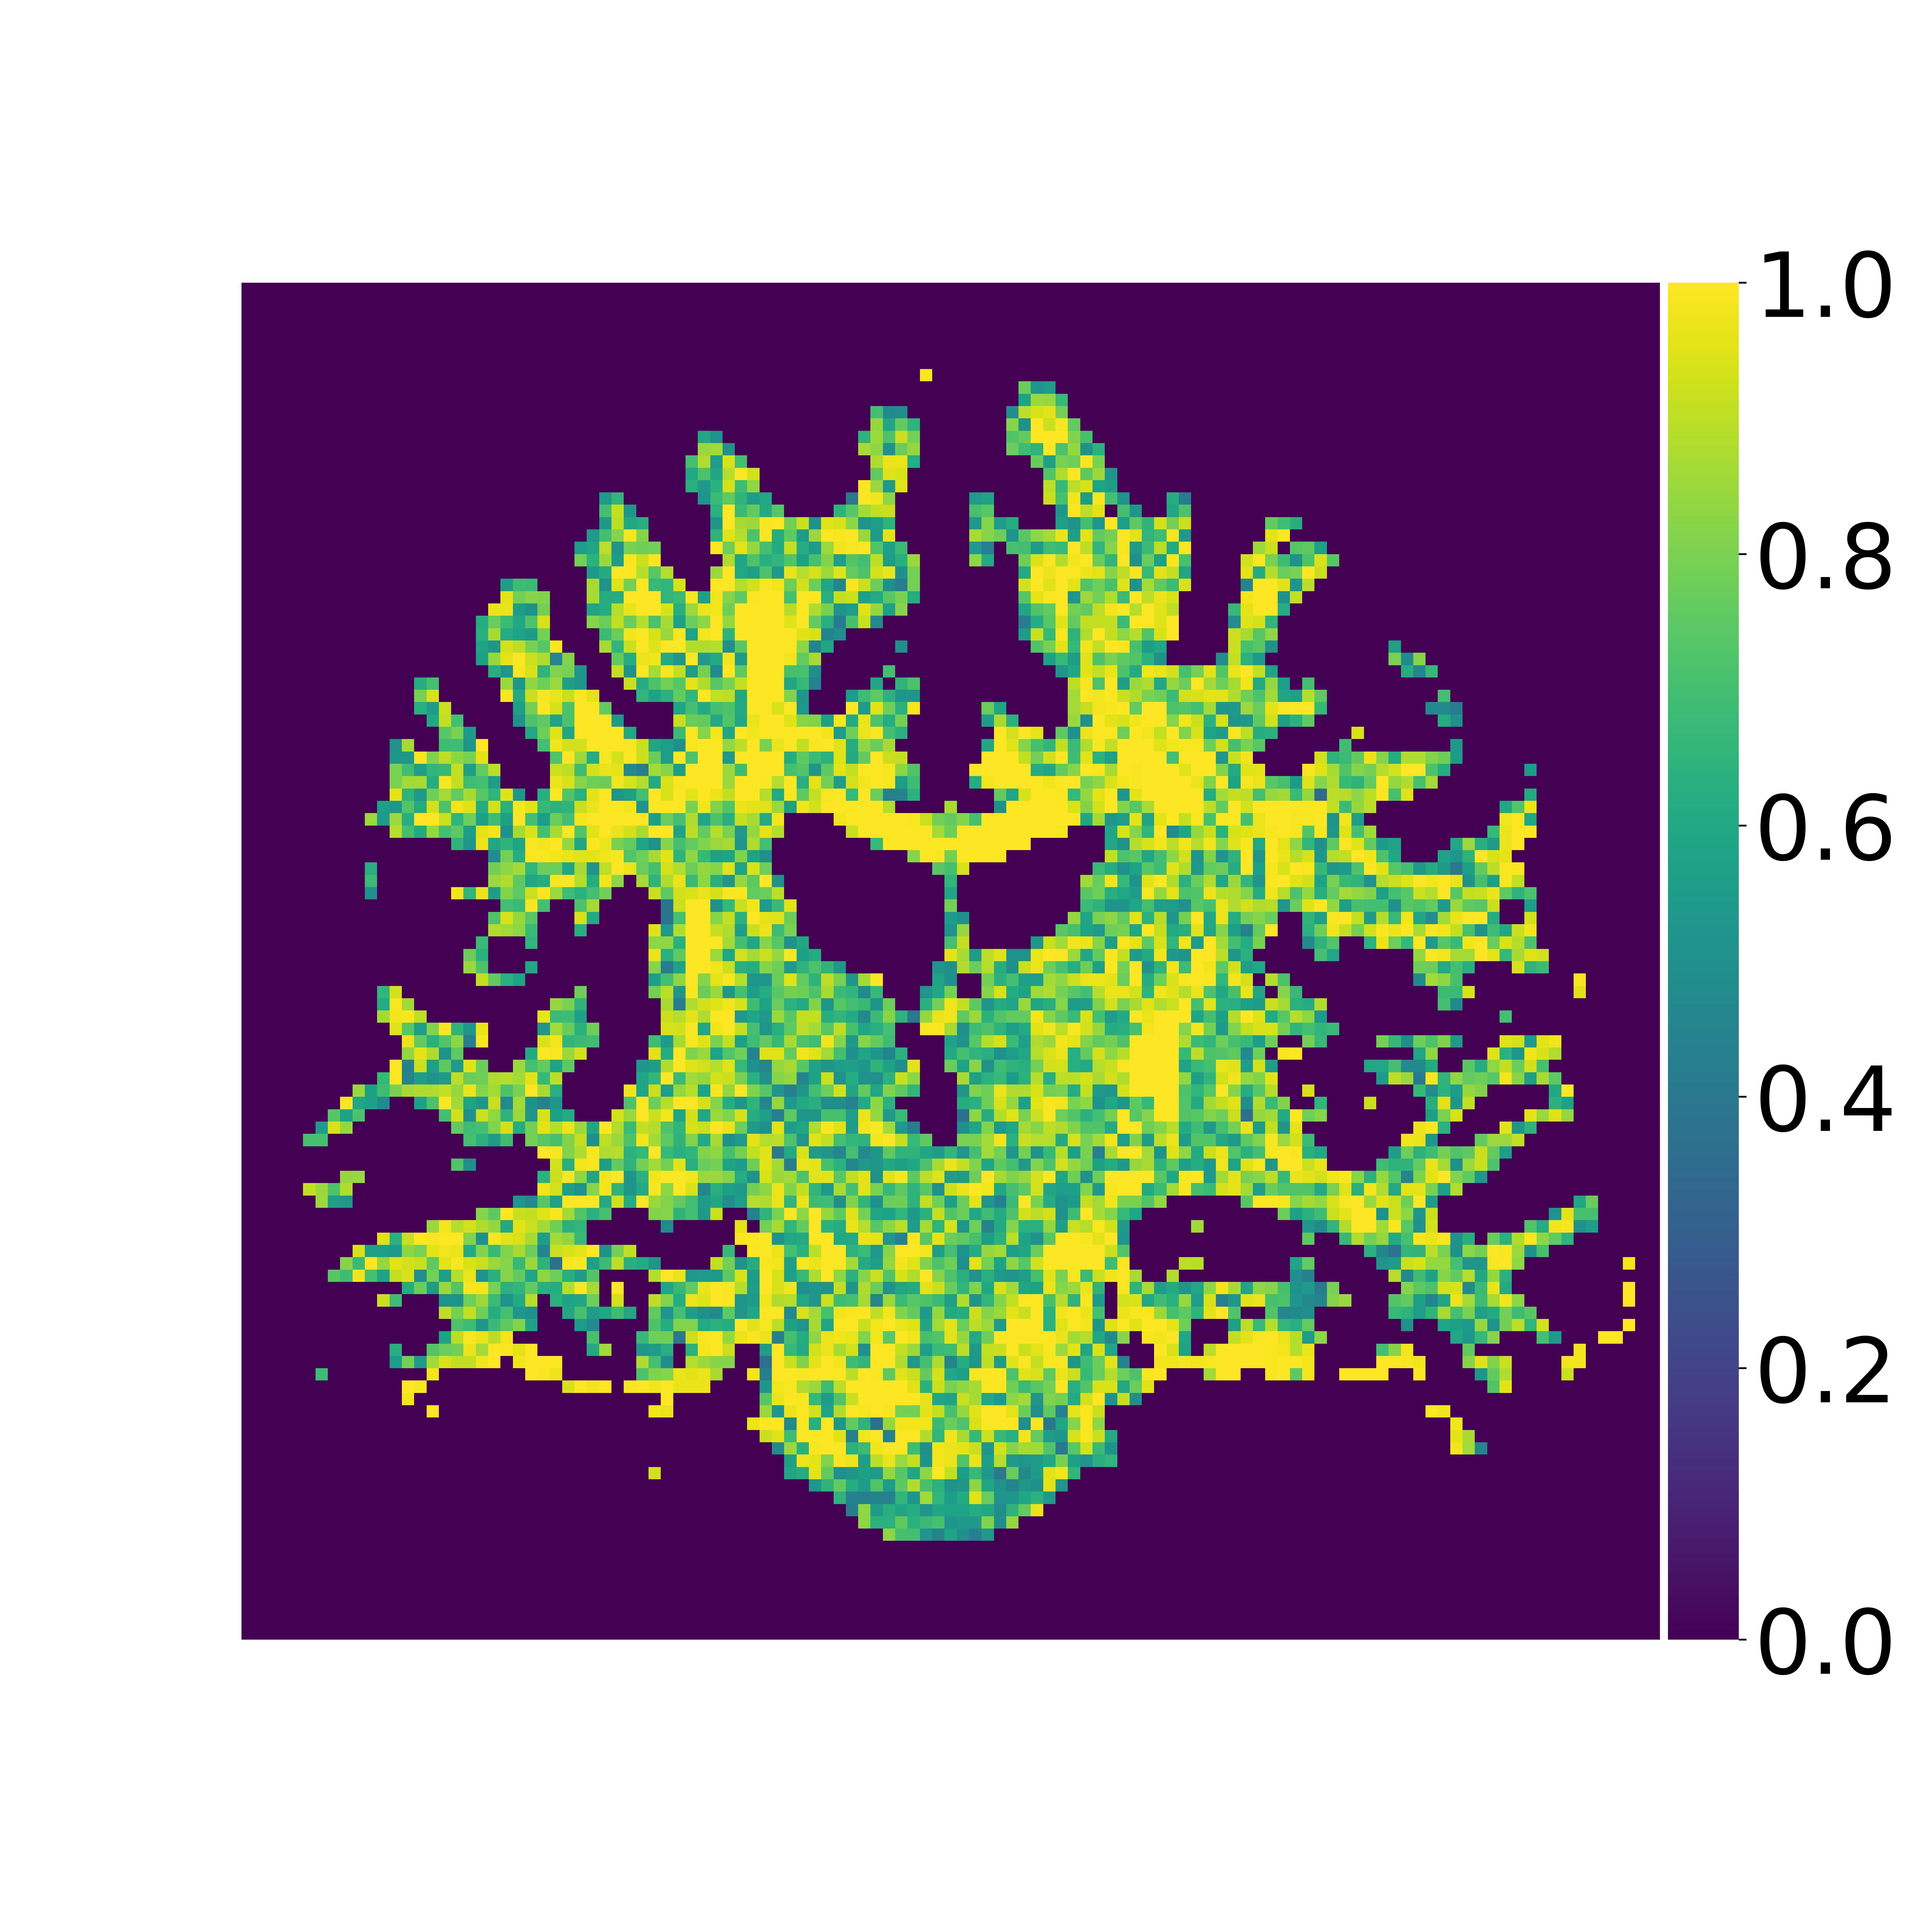
\includegraphics[width=\linewidth]{uncertainty-bootstrap}
		\caption{Fraction of bootstraps which selected the number of fibers in (b).}
		\label{fig:selected-uncertainty:unc}
	\end{subfigure}
	\caption{Small differences between model selection without bootstrapping (a) and the most frequently selected model under bootstrapping (b) indicate that data uncertainty also has a certain effect on the selected model. The stability of model selection under bootstrapping (d) correlates well with the confidence derived from our Bayesian framework (c).}
	\label{fig:selected-uncertainty}
\end{figure*}

We describe the variability that arises from noise in the dMRI measurement as data uncertainty. Taking measurements repeatedly is a natural way to estimate it, but is usually not feasible in practice. Therefore, different bootstrapping techniques have been established to estimate data uncertainty based on a single DTI or HARDI acquisition \cite{Chung:2006,Jones:2008}.

We summarize one such bootstrapping approach in Section~\ref{sec:wild-bootstrap}, and use it in two ways: In Section~\ref{sec:data-vs-model-uncertainty}, we investigate the interaction between data and model uncertainty, by studying the variance of the selected model under bootstrapping. In Section~\ref{sec:bootstrap-consensus}, we define a bootstrap consensus for the joint reduction of data and measurement uncertainty. As a by-product, this allows us to investigate the effect of model selection and averaging on the variability of fiber direction estimates in Section~\ref{sec:vis-uncertainty-reduction}.

\subsection{Wild Bootstrapping}
\label{sec:wild-bootstrap}
We use wild bootstrapping to evaluate the impact of measurement noise. It is a straightforward way to
resample the original measurements without repeating the measurement process, and has been used widely in the context of dMRI
\cite{Jones:2008,Schultz:EuroVis2013,Siddiqui:2021}.

Wild bootstrapping uses model residuals to estimate noise. We combine it with the fODF tensor framework from Section~\ref{sec:background} by fitting an initial fODF
$\hat{\mathcal{T}}$ via Eq. (\ref{eq:sd-min}), and calculating the residual 
\[ \hat{\varepsilon} = S - M\hat{\mathcal{T}} .\] 
A new bootstrap realization is calculated by 
\[ y^{*} = M\hat{\mathcal{T}}  + \hat{\varepsilon}\added{\odot} v , \]
where $v$ denotes a random draw from the $n$ dimensional Rademacher distribution
\[ f \left( \added{\mathbf{k}_i} \right) \coloneqq  \begin{cases} \nicefrac{1}{2} \text{ if }
		\mathbf{k}_i=-1 \\
		\nicefrac{1}{2} \text{ if } \mathbf{k}_i=1 \\
		0 \text { otherwise } 
\end{cases} \text{ for } i \in \left\{ 1\dots n \right\} . \]
\added{and $\odot$ denotes component-wise multiplication.}

This process is repeated $m$ times to create a sample of $m$ bootstraps. For each bootstrap realization, we fit a new fODF and compute its low-rank approximations.

%For each sampled fODF we calculate the low-rank approximation of rank $3$
%and with the obtained residuals also the selection and average model as it is
%described in the previous section.

\subsection{Interaction Between Data and Model Uncertainty}
\label{sec:data-vs-model-uncertainty}

We hypothesized that data and model uncertainty interact in the sense that, in many voxels, the effect of measurement noise is sufficient to change the selected fiber number. We were also interested in the extent to which the frequencies with which different ranks are selected under bootstrapping agree with the probabilities that are assigned by our Bayesian model.

Therefore, we took 100 bootstraps and applied model
selection to all of them. Comparing the most
likely number of fibers in the original data (Fig.~\ref{fig:selected-uncertainty:rank-original}) to the number that is most frequently selected over all bootstraps (Fig.~\ref{fig:selected-uncertainty:rank}) already reveals a certain amount of variability: In $14.1\%$ of the voxels within the white matter, the selected rank differs
by $1$; in $0.8\%$, it differs by $2$.

The probability of the most likely number of fibers according to Eq.~(\ref{eq:Bayes}) is
shown in Fig.~\ref{fig:selected-uncertainty:unc-original}, next to the fraction of bootstraps that agreed on the most frequently selected number in Fig.~\ref{fig:selected-uncertainty:unc}. Visually, we find a remarkable agreement between the regions in which our Bayesian framework has a high confidence in its choice (high values in c), and the regions in which the choice is stable under bootstrapping (high values in d). We believe that this provides further empirical support for the framework proposed in Section~\ref{sec:model-comparison}.

\subsection{Bootstrap Consensus}
\label{sec:bootstrap-consensus}
\begin{figure*}[t]
	\centering
	\begin{subfigure}[b]{0.32\linewidth}
		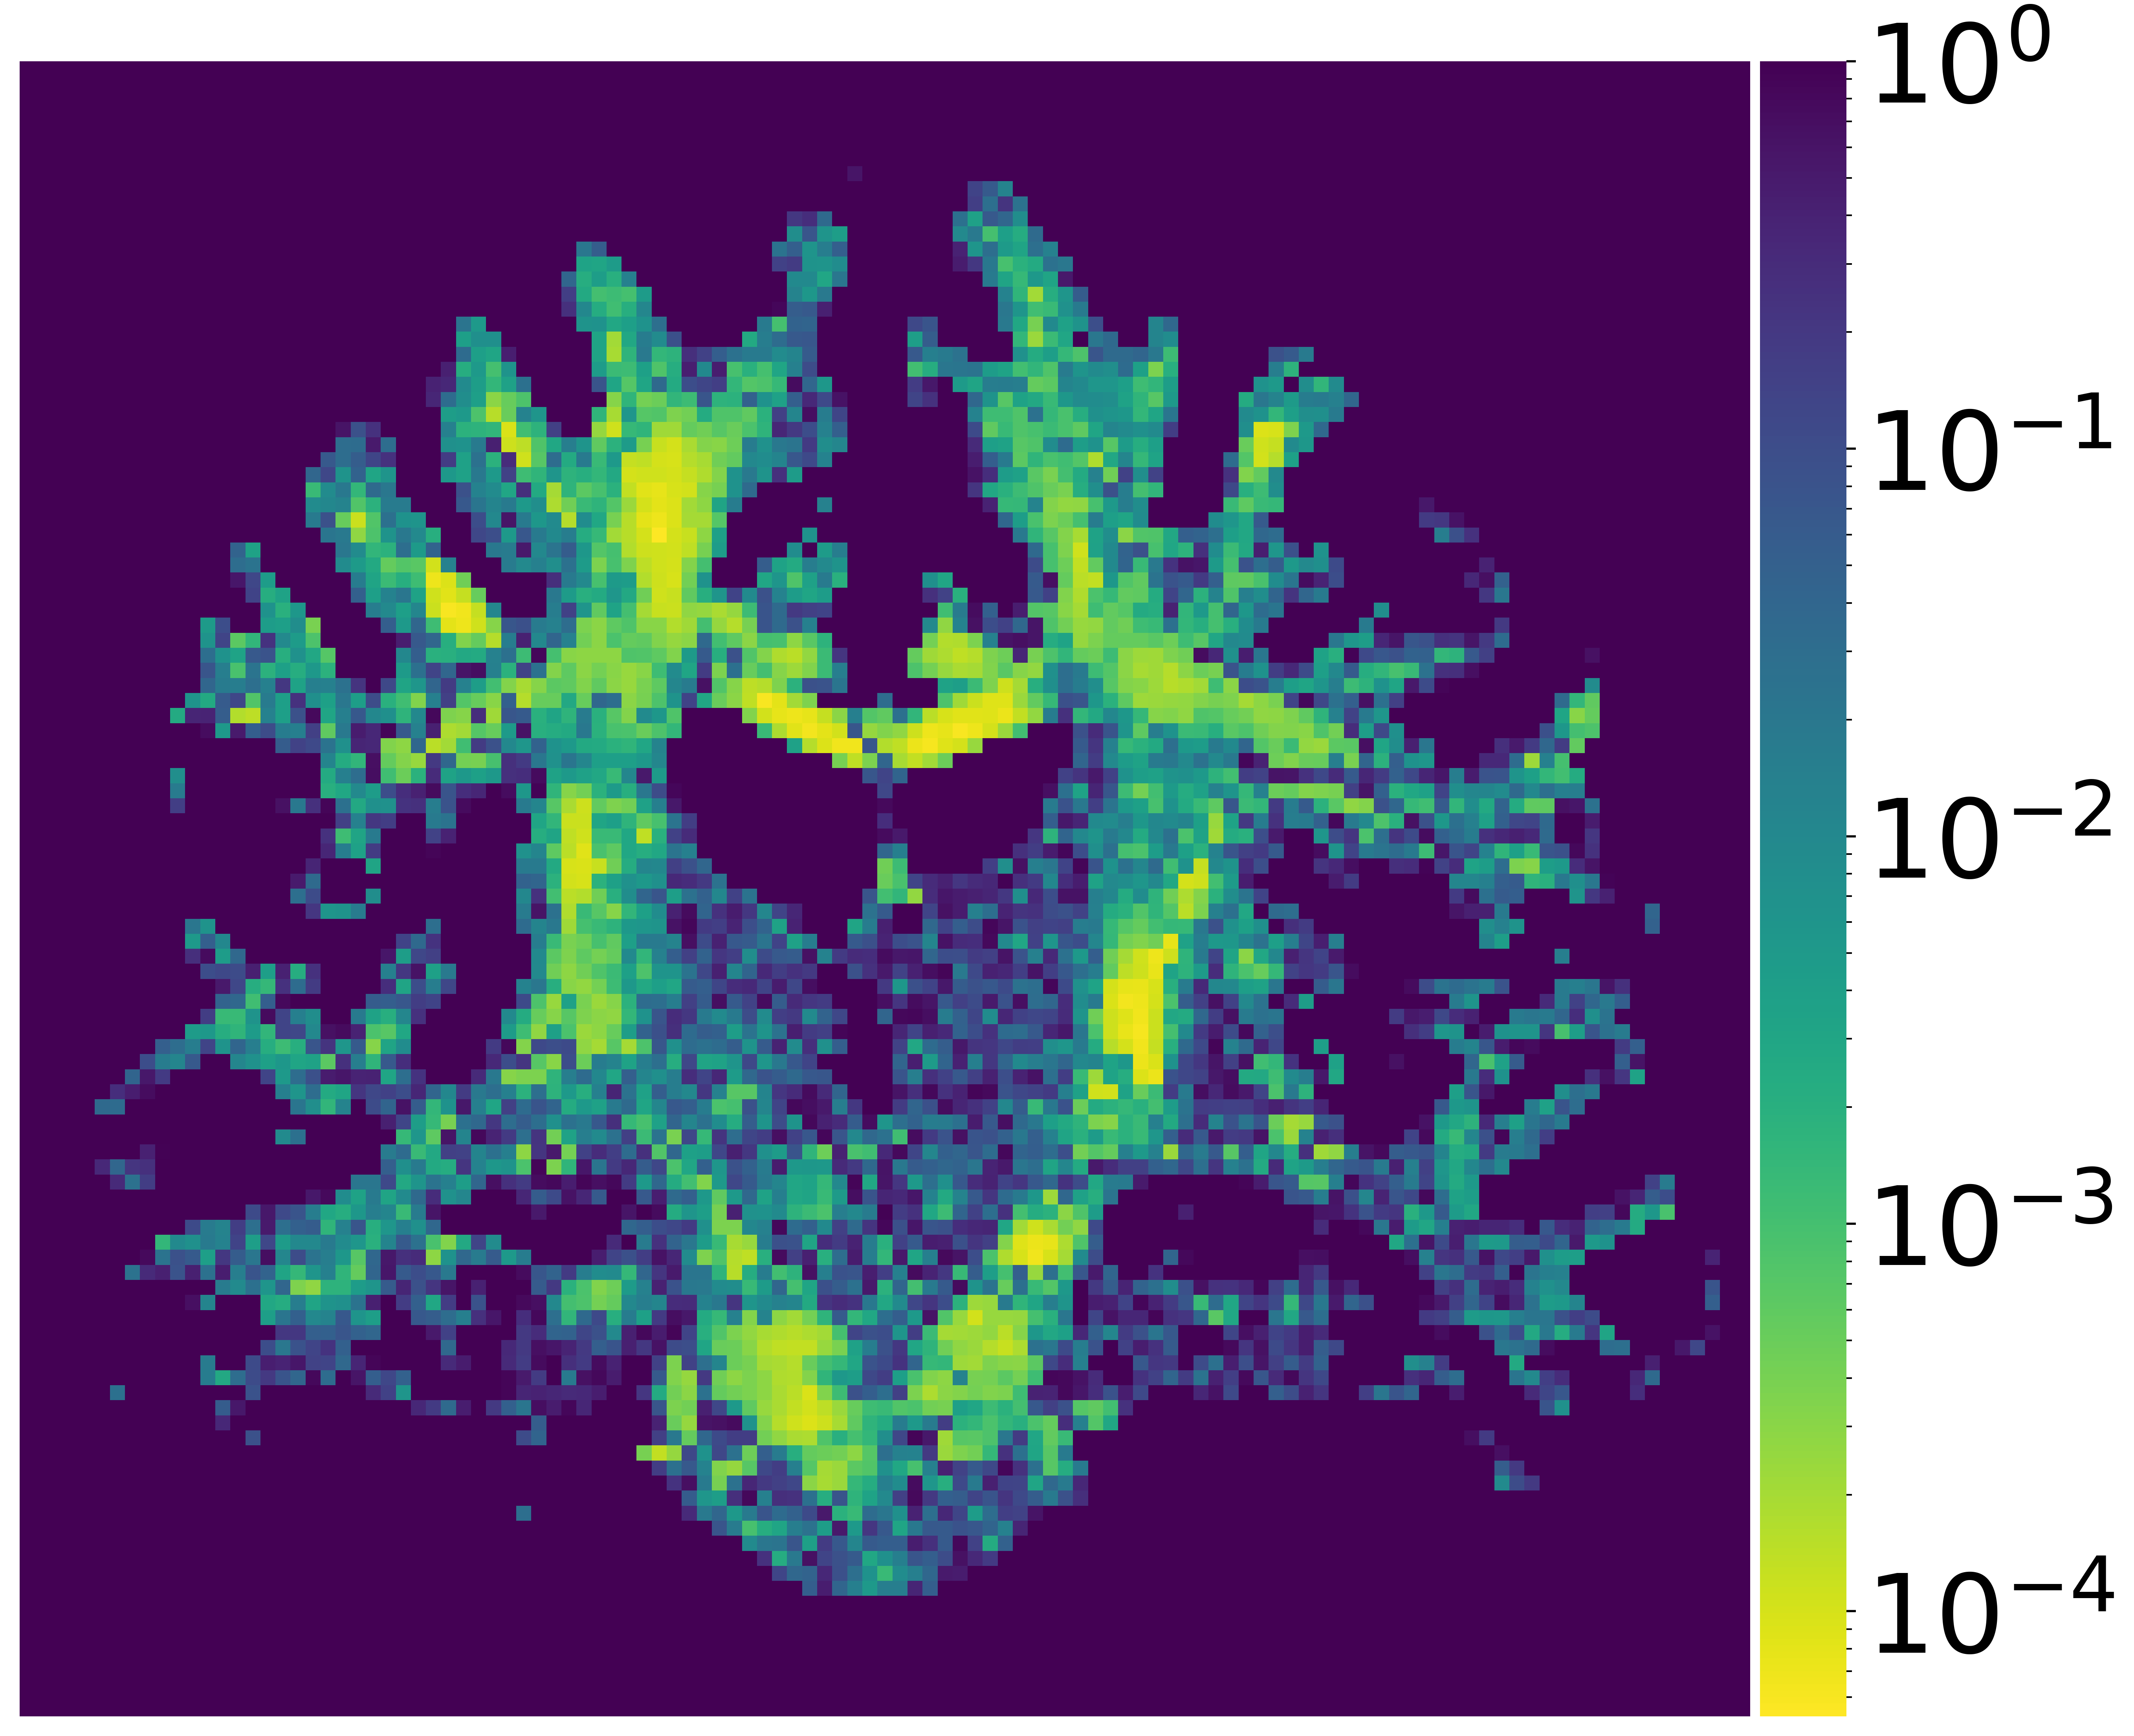
\includegraphics[width=\linewidth]{sel-bootstrap-maindir}
		\caption{Model Selection}
		
	\end{subfigure}
        \hspace{0.01\linewidth}
	\begin{subfigure}[b]{0.32\linewidth}
		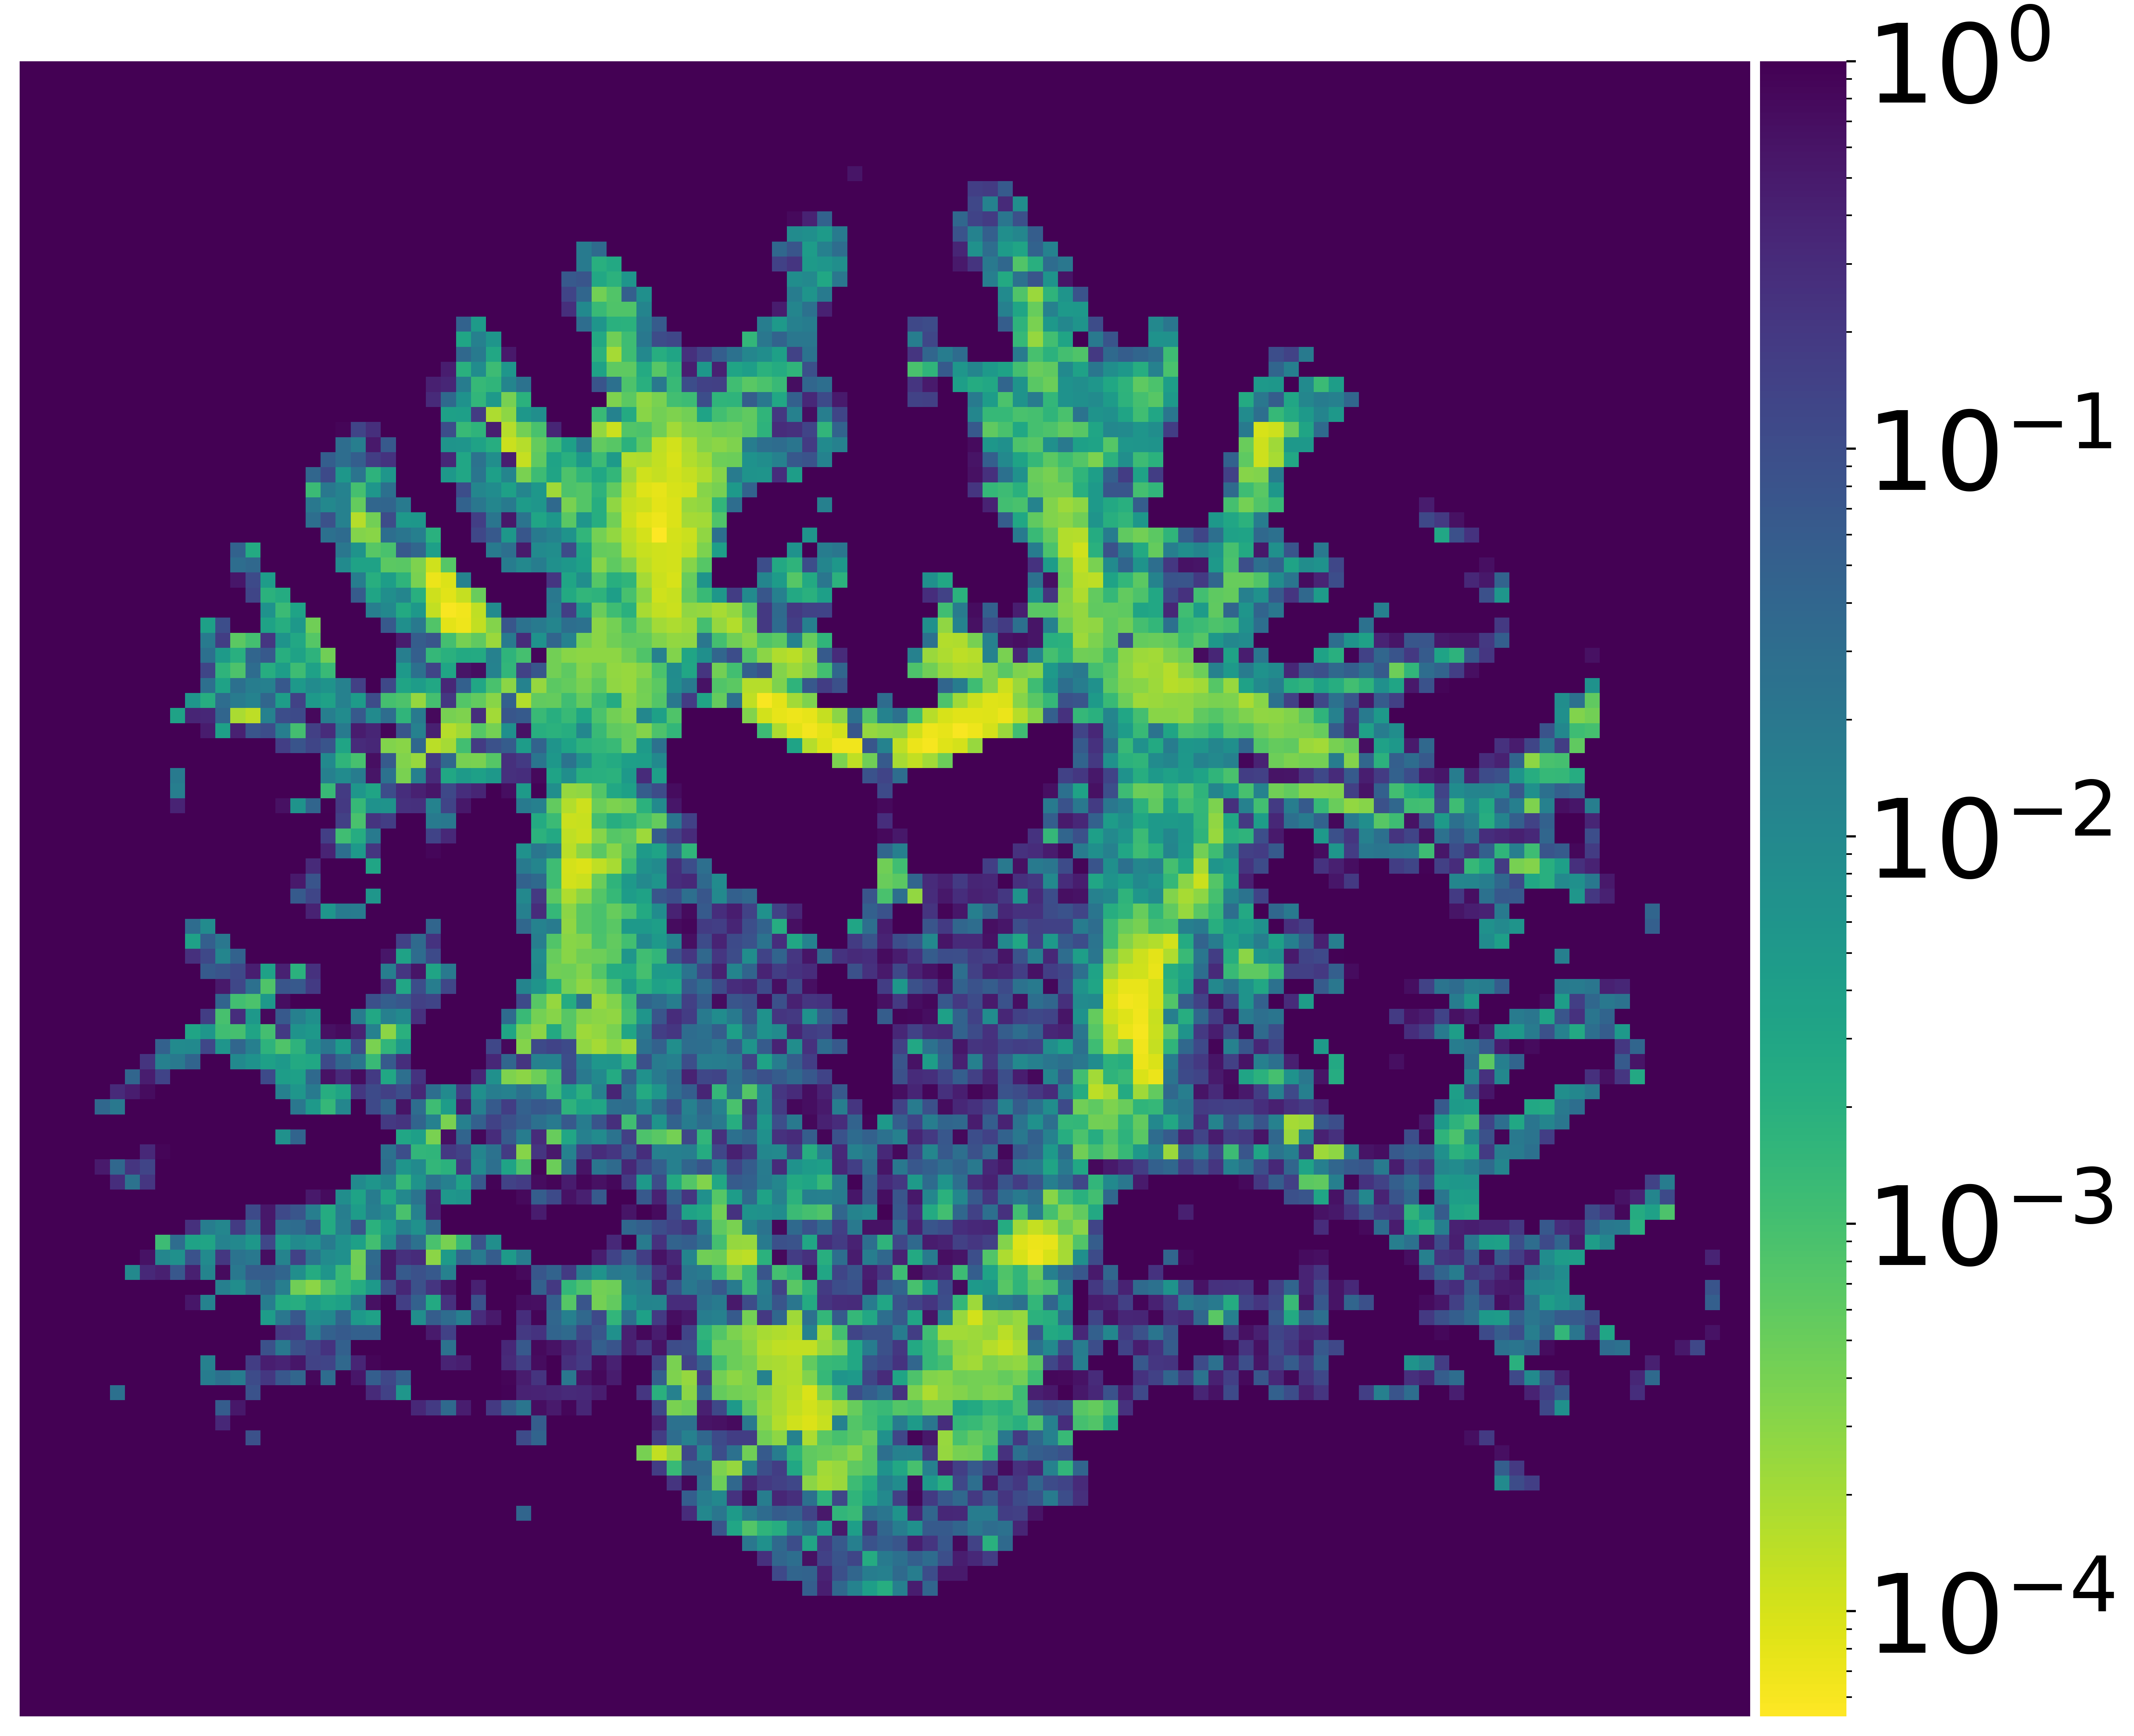
\includegraphics[width=\linewidth]{avg-bootstrap-maindir}
		\caption{Model Averaging}
	\end{subfigure}
        \hspace{0.01\linewidth}
	\begin{subfigure}[b]{0.32\linewidth}
		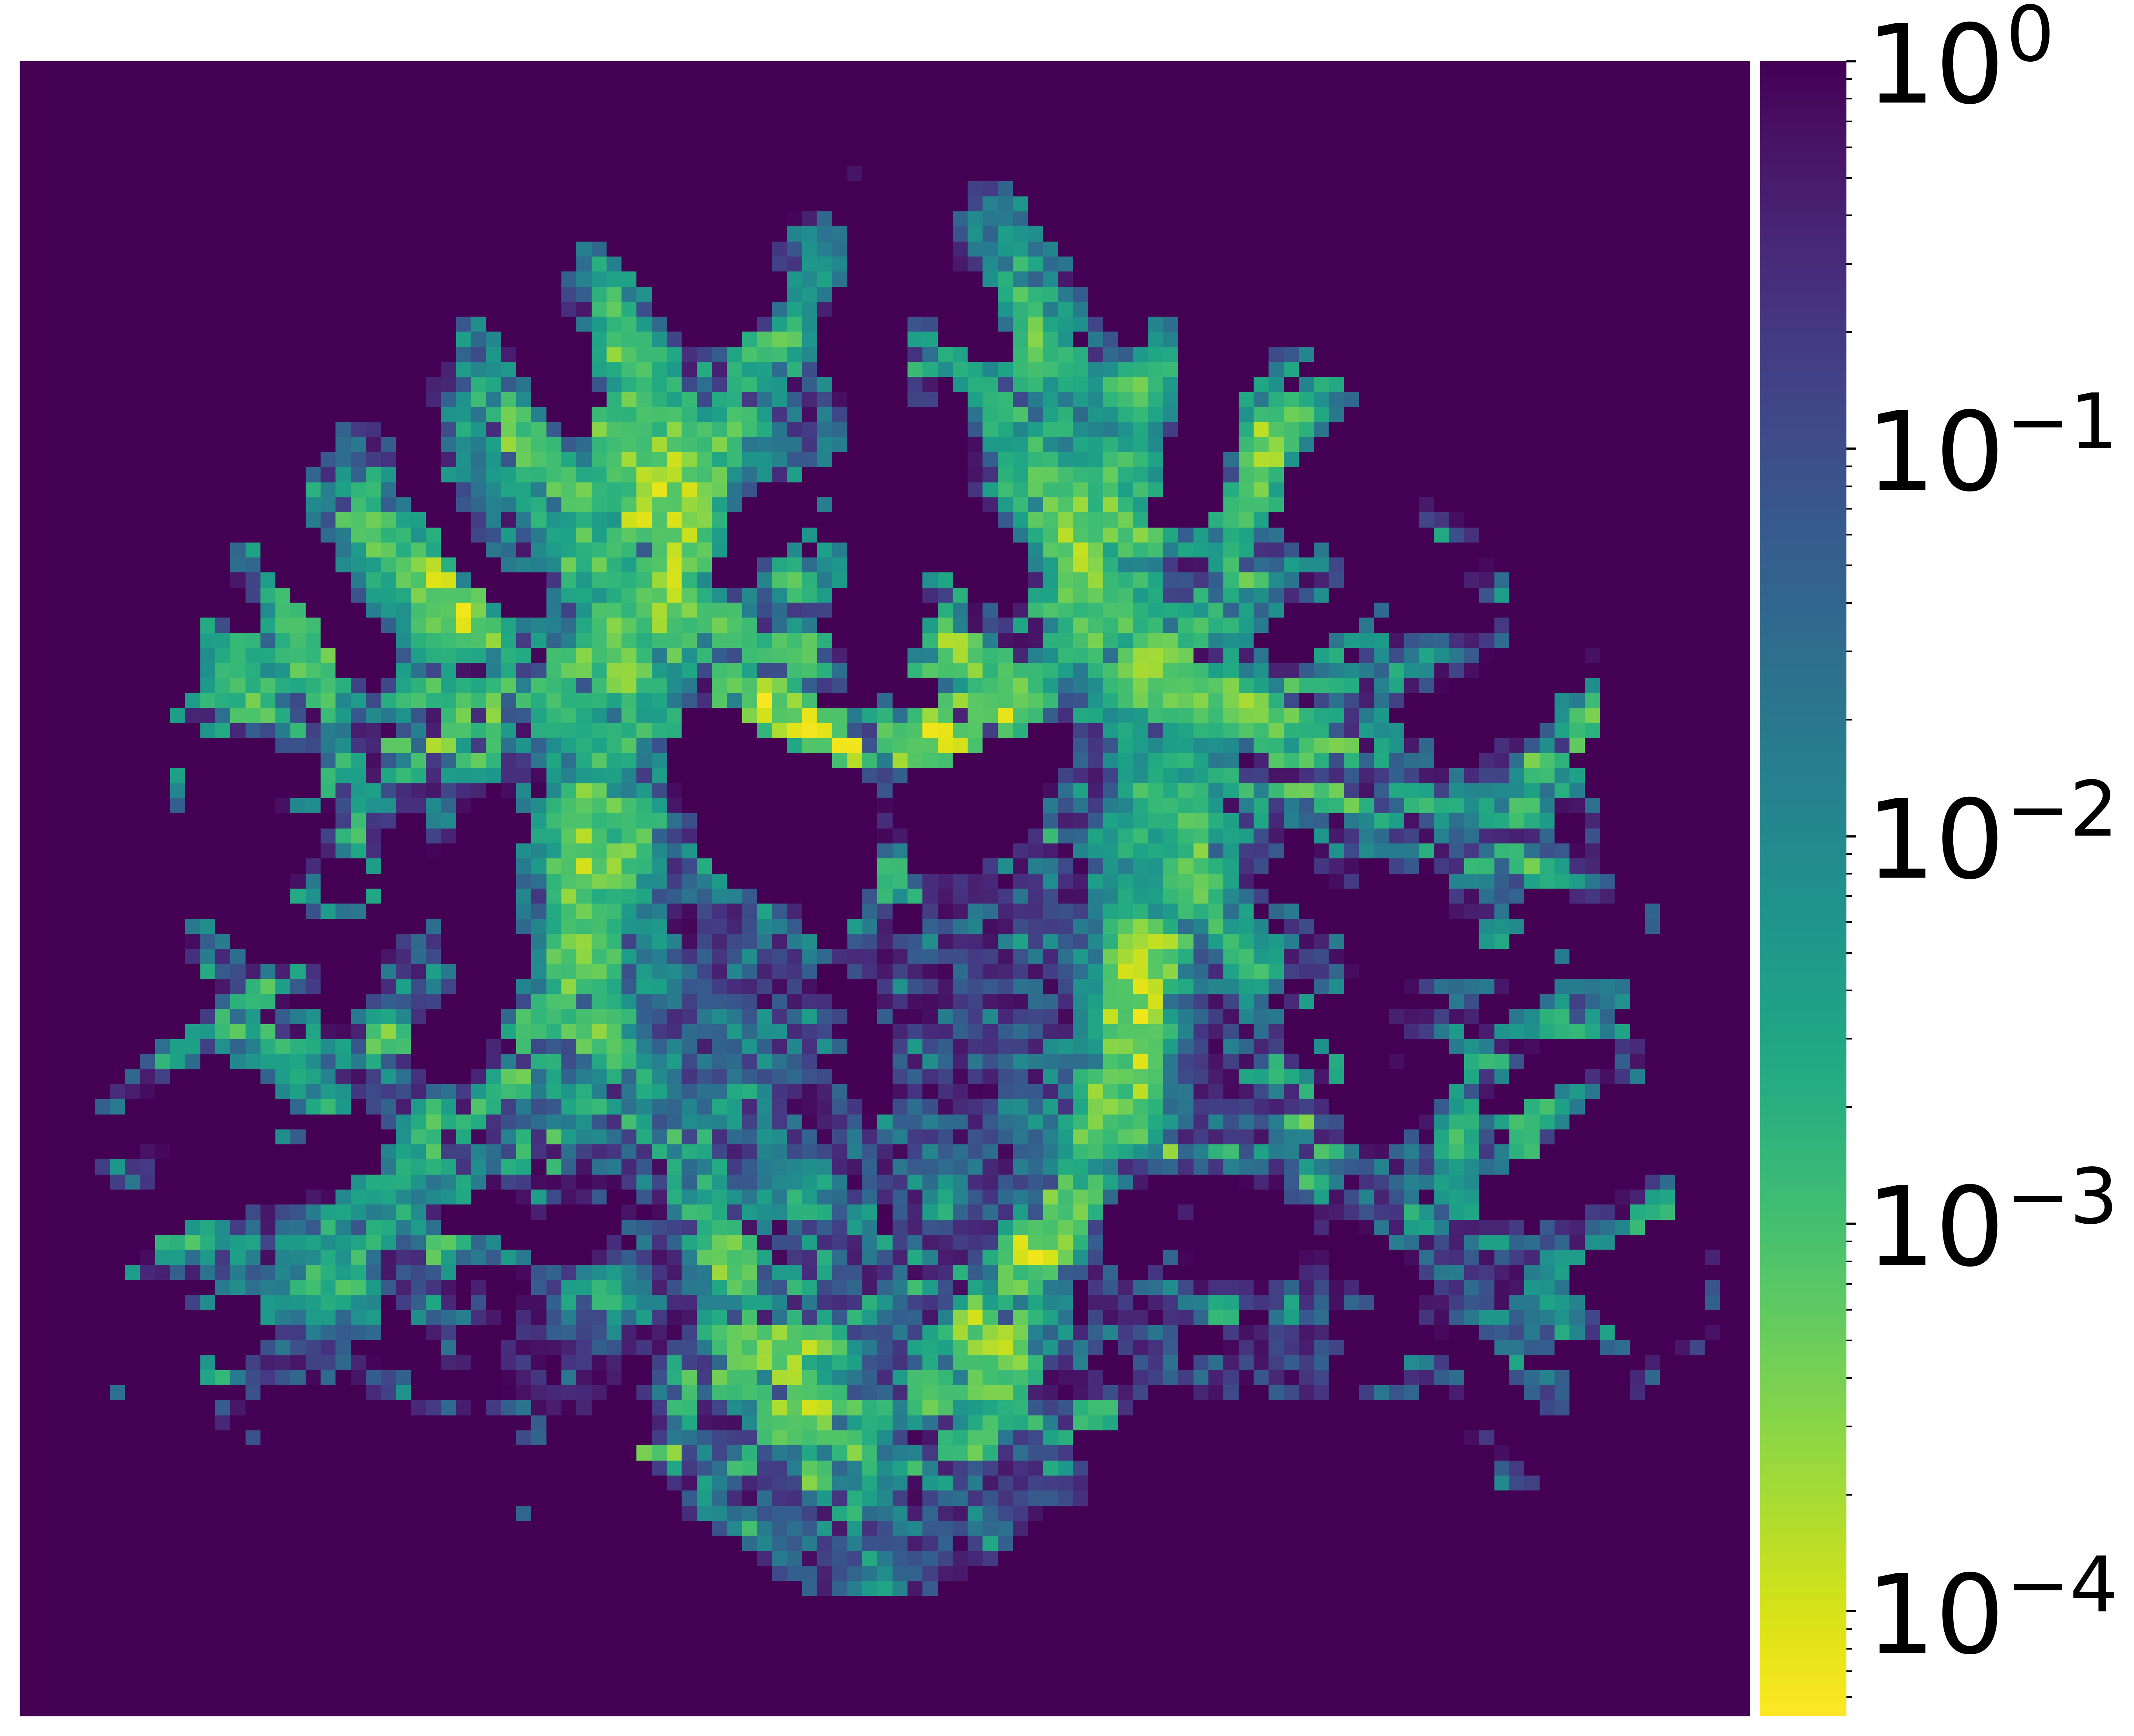
\includegraphics[width=\linewidth]{rank-bootstrap-maindir}
		\caption{Rank-3 Approximation}
	\end{subfigure}

	\caption{Mapping orientation dispersion of the principal fiber
		direction under bootstrapping confirms that the dispersion in the rank-$3$
result is higher than with model selection or averaging, indicating their ability to decrease susceptibility to noise.}
	\label{fig:dispersion}
\end{figure*}

In analogy to how the model averaging in Section~\ref{sec:computing-tracking-directions} reduces model uncertainty by fusing information from alternative models, we derive a bootstrap consensus that fuses information from all bootstraps. We emphasize that this differs from the traditional use of bootstrapping in probabilistic tractography, where bootstrap samples produce a distribution of streamlines from a common seed \cite{Jones:2008,Jeurissen:2011}. Instead of estimating data uncertainty, our bootstrap consensus aims to reduce its effect. Due to the interaction between data and model uncertainty that was observed in Fig.~\ref{fig:selected-uncertainty}, it can also be expected to jointly reduce model uncertainty.

The bootstrap consensus is formed by clustering the directions from all bootstraps into groups, and taking the group means as the final tracking directions. Specifically, we assign the $n_i$ directions from the $i$th bootstrap to $m$ groups, where we set $m=3$ as the maximum number of fibers we are willing to consider. Due to the large number of bootstraps, an enumeration of all possible assignments that guarantees a global optimum, as it could be used in Section~\ref{sec:computing-tracking-directions}, is no longer feasible.

Instead, we initialize the reference
directions for each group with a rank-$3$ approximation of the original data. Now, the
directions from each bootstrap are assigned to the groups such that the sum of
distances between the group
reference and the directions are minimized over all possible assignments. Formally, we minimize the objective function 
\begin{align}
  \label{eq:matching-cost}
	T : \text{Sym} \left( n \right) & \mapsto \mathbb{R}_+ \nonumber \\
	Z & \rightarrow \sum \| \sgn \left( \langle \mathbf{v}_{Z\left( i
	\right)}, \bar{\mathbf{v}}_i \rangle \right) \mathbf{v}_{Z\left( i
	\right)} - \bar{\mathbf{v}}_i\| ,  
\end{align} 
where $\text{Sym}\left( n \right)$ denotes the symmetric group, 
$\bar{\mathbf{v}}_i$ denotes
the reference direction, $\mathbf{v}_i$ denotes the direction from the
bootstrap.
% I think the following contradicts the initialization above:
% To prevent wrong assignments if only one reference
%direction is initialized we first assign the direction from the bootstrap with
%the  highest fiber count to the
%groups and update the uninitialized reference directions with the assignments.
%Note that this does not necessary lead to a global optimum, but is in most cases
%close to the optimum. 

\subsection{Visualizing the Uncertainty in Fiber Directions}
\label{sec:vis-uncertainty-reduction}

Our main motivation for using model selection or averaging instead of always
extracting the maximum number of fibers is that we expect it to reduce variance
in the true fiber estimates. The clustering that we perform to compute the
bootstrap consensus can be used to quantify and visualize this effect.  The Watson distribution is defined as  \cite{jupp_mardia_1999}
\begin{align*}
	f : \mathbb{S}^2 & \longrightarrow  \mathbb{R}_+ \\
	\mathbf{x} & \longmapsto \added{\frac{1}{M \left( \frac{1}{2}, \frac{3}{2} , \kappa \right)}} \exp \left(  \kappa
	\left( \mathbf{\mu}^T \mathbf{x} \right)^2 
	\right) 	,  
\end{align*}
where $\kappa$ is the dispersion parameter, $\| \mathbf{\mu} \| = 1$ the
mean direction, and \added{the normalizing factor involves the confluent
	hypergeometric function $M$ \cite{Kummer:1837}. To estimate the
	dispersion $\kappa$ we used the maximum likelihood estimator \cite{jupp_mardia_1999}, which
allowed us to determine $\kappa$ via Newton optimization.}

We use the Watson distribution for two reasons: First, it is antipodally symmetric,
which fits the fact that in Eq.~(\ref{eq:low-rank}), directions $\pm \mathbf{v}$
are indistinguishable. Second, its dispersion parameter $\kappa$ allows us to quantify the variability in the fiber directions within each group. $\kappa$ can be re-parameterized to obtain an orientation dispersion index
\[ \mathrm{OD} = \frac{2}{\pi} \arctan \left( \frac{1}{\kappa} \right) \]
that is normalized to $(0,1)$ and indicates higher variability with higher values \cite{dispersionParameter}.

Fig.~\ref{fig:dispersion} visualizes orientation dispersion of the primary fiber that was estimated with model selection, model averaging, or a rank-3 approximation. In particular in the regions in which model selection picks a single fiber (cf.\ Fig.~\ref{fig:selected-uncertainty}; this includes parts of the corpus callosum and corticospinal tract), this results in lower dispersion 
compared to the rank-$3$ model, confirming our expectation that estimating a single fiber direction is less susceptible to noise than estimating multiple directions from the same data. The same regions still have reduced dispersion after model averaging, confirming its effectiveness for uncertainty reduction.

% Maybe this could go into the discussion part later on:
%We conclude that average model fuses the stability from the selection model in
%the mean direction and also the flexibility of the rank $3$ model, which can be
%important in crossing regions.
%Therefore, we assume that the impact to the average and rank $3$ model is lower
%than to the selection model since we increase the flexibility by introducing
%more directions into the consensus selection model. 



%%% Local Variables:
%%% mode: latex
%%% TeX-master: "../main"
%%% End:
